% #3589 | Archive/SP_KhoLatex/ID6_old/2D2B4-7.tex | mã gốc 2D2B4-7
\begin{ex}%[Thi thử L1, Star Education HCM, 2019]%[Nguyễn Ngọc Dũng, dự án 12EX6]%[2D2B4-7]
\immini{
Cho $a$, $b$, $c$ là ba số thực dương và khác $1$. Đồ thị các hàm số $y=\log_a x$, $y=\log_b x$, $y=\log_c x$ được cho trong hình vẽ bên. Mệnh đề nào dưới đây là mệnh đề đúng?
\motcot
{$ a<b<c$}
{\True $ c<a<b$}
{$ c<b<a$}
{$ b<c<a$}
}{
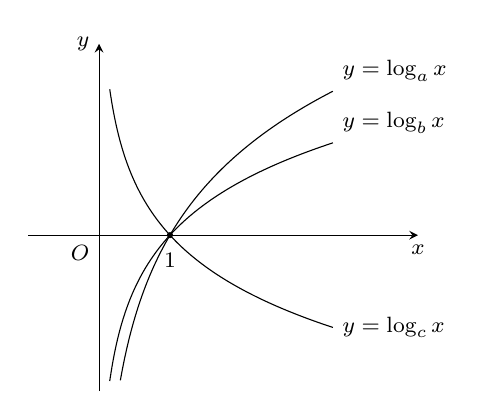
\begin{tikzpicture}[>=stealth, scale =0.9, font=\footnotesize]
\draw[->] (-1,0)--(4.5,0) node[below]{$x$};
\draw[->] (0,-2.2)--(0,2.7) node[left]{$y$} ;
\draw[fill=black] (0,0) node[below left]{$O$} (1,0) circle(1pt) node[below, yshift=-1mm]{$1$};
\draw[samples=100, smooth, domain=0.15:3.3] plot(\x,{ln((\x))/ln(2.5)}) node[above right]{$y=\log_b x$};
\draw[samples=100, smooth, domain=0.3:3.3] plot(\x,{ln((\x))/ln(1.8)})node[above right]{$y=\log_a x$};
\draw[samples=100, smooth, domain=0.15:3.3] plot(\x,{ln((\x))/ln(0.4)}) node[right]{$y=\log_c x$};
\end{tikzpicture}
}
\loigiai{
\immini{
Đường thẳng $y=1$ cắt đồ thị tại các điểm có hoành độ như hình vẽ, từ đó suy ra $c<a<b$.
}{
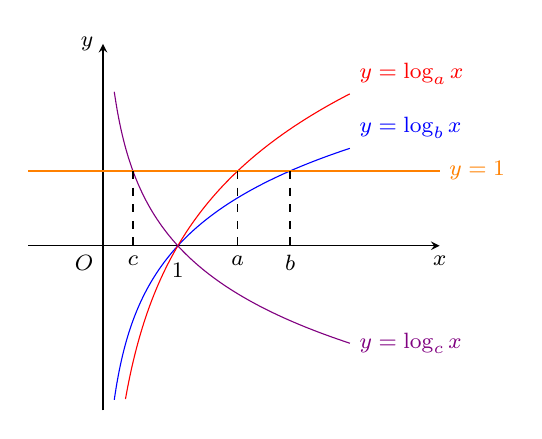
\begin{tikzpicture}[>=stealth, scale =0.95, font=\footnotesize]
\draw[->] (-1,0)--(4.5,0) node[below]{$x$};
\draw[->] (0,-2.2)--(0,2.7) node[left]{$y$} ;
\draw (0,0) node[below left]{$O$} (1,0) node[below, yshift=-1mm]{$1$};
\draw[samples=100, smooth, domain=0.15:3.3, color=blue] plot(\x,{ln((\x))/ln(2.5)}) node[above right]{$y=\log_b x$};
\draw[samples=100, smooth, domain=0.3:3.3, color=red] plot(\x,{ln((\x))/ln(1.8)})node[above right]{$y=\log_a x$};
\draw[samples=100, smooth, domain=0.15:3.3, color=violet] plot(\x,{ln((\x))/ln(0.4)}) node[right]{$y=\log_c x$};
\draw[color=orange] (-1,1)--(4.5,1) node[right]{$y=1$};
\draw (2.5,0) node[below]{$b$} (1.8,0) node[below]{$a$} (0.4,0) node[below]{$c$};
\draw[dashed] (0.4,1)--(0.4,0) (1.8,1)--(1.8,0) (2.5,1)--(2.5,0);
\end{tikzpicture}
}}
\end{ex}

% #3596 | Archive/SP_KhoLatex/ID6_old/2D2B2-3.tex | mã gốc 2D2B2-3
\begin{ex}%[GHK2, THPT Nghèn - Hà Tĩnh, 2019]%[Nguyễn Nguyễn Quang Dũng, dự án 12-EX-5-2019]%[2D2B2-3]
Cho các số thực $\alpha$ và $\beta$. Đồ thị các hàm số $y=x^\alpha,\ y=x^\beta$ trên khoảng $(0;+\infty)$ như hình vẽ bên, trong đó đường \textbf{đậm hơn} là đồ thị hàm số $y=x^\beta$. Mệnh đề nào dưới đây đúng?
\immini{\motcot
{$0<\beta<\alpha<1$}
{$\alpha<0<\beta<1$}
{\True $0<\beta<1<\alpha$}
{$\beta<0<1<\alpha$}}
{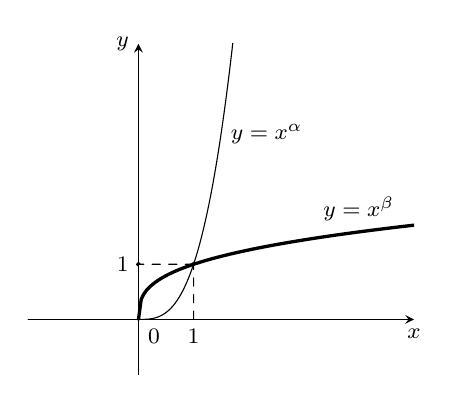
\begin{tikzpicture}[scale=0.7, font=\footnotesize, line join=round, line cap=round, >=stealth]
\draw[->] (-2,0)--(5,0) node [below] {\footnotesize $x$};
\draw[->] (0,-1)--(0,5) node [left] {\footnotesize $y$};
\def\f[#1]{(#1)^3};
\def\g[#1]{(#1)^(1/3)};
\clip (-2,-1) rectangle (5,5);
\draw [domain=0:2,samples=100] plot (\x,{\f[\x]});
\path [domain=0:1.5,samples=100] plot (\x,{\f[\x]})node [right] {\footnotesize $y=x^\alpha$};
\draw [domain=0:5,samples=100,line width =1.2pt] plot (\x,{\g[\x]});
\path [domain=0:4,samples=100,line width =1.2pt] plot (\x,{\g[\x]}) node [above] {\footnotesize $y=x^\beta$};
\foreach \x in {1} {
\pgfmathsetmacro\fx{\f[\x]};
\draw [dashed](\x,0)--(\x,\fx)circle(1pt)--(0,\fx)circle(1pt);}
\draw (1,0)node [below] {$1$}(0,0)node [below right] {$0$}(0,1)node [left] {$1$};
\end{tikzpicture}}
\loigiai{
\immini{
Do hai hàm số $y=x^\alpha$ và $y=x^\beta$ cùng đồng biến trên $(0;+\infty)\\
\Rightarrow \alpha>0,\ \beta>0$.\\
Xét tại $x=2$, theo đồ thị ta có
\begin{itemize}
\item $2^\beta < 2^1\Leftrightarrow \beta <1$.\tagEX{1}
 \item $2^\alpha>2^1\Leftrightarrow \alpha >1$.\tagEX{2}
\end{itemize}
Từ $(1)$ và $(2)\Rightarrow 0<\beta<1<\alpha$.}
{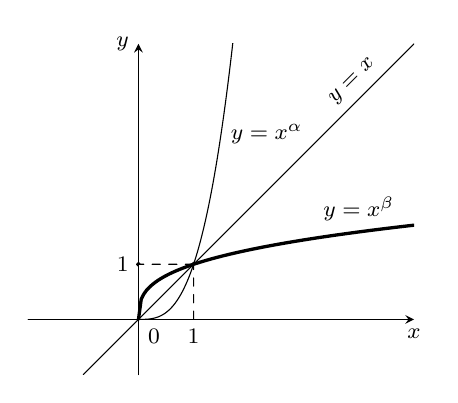
\begin{tikzpicture}[scale=0.7, font=\footnotesize, line join=round, line cap=round, >=stealth]
\draw[->] (-2,0)--(5,0) node [below] {\footnotesize $x$};
\draw[->] (0,-1)--(0,5) node [left] {\footnotesize $y$};
\def\f[#1]{(#1)^(3)};
\def\g[#1]{(#1)^(1/3)};
\clip (-2,-1) rectangle (5,5);
\draw [domain=0:2,samples=100] plot (\x,{\f[\x]});
\path [domain=0:1.5,samples=100] plot (\x,{\f[\x]})node [right] {\footnotesize $y=x^\alpha$};
\draw [domain=0:5,samples=100,line width =1.2pt] plot (\x,{\g[\x]});
\path [domain=0:4,samples=100,line width =1.2pt] plot (\x,{\g[\x]}) node [above] {\footnotesize $y=x^\beta$};
\foreach \x in {1} {
\pgfmathsetmacro\fx{\f[\x]};
\draw [dashed](\x,0)--(\x,\fx)circle(1pt)--(0,\fx)circle(1pt);}
\draw (1,0)node [below] {$1$}(0,0)node [below right] {$0$}(0,1)node [left] {$1$};
\draw (-1,-1)--(5,5)node[pos=0.85,above,rotate=45]{$y=x$};
\end{tikzpicture}}}
%Bạn đã lấy 1 lần
\end{ex}

% #3600 | Archive/SP_KhoLatex/ID6_old/2D2B4-3.tex | mã gốc 2D2B4-3
\begin{ex}%[Thi thử L4, THPT chuyên ĐHSP Hà Nội, 2018]%[Nguyễn Hữu Nhân, dự án (12EX-11)]%[2D2B4-3]
	Hình bên là đồ thị của hàm số nào trong các hàm số sau đây?
	\immini{
	\haicot
	{\True $y=2^x$}
	{$y=(0,8)^x$}
	{$y=\log_2x$}
	{$y=\log_{0,5}x$}}
	{\begin{tikzpicture}[>=stealth,scale=0.7, line join = round, line cap = round]
	\draw[->] (-2,0) -- (0,0) node[below left] {\footnotesize $O$} -- (3,0) node[below] {\footnotesize $x$};
	\draw[->] (0,-0.5) -- (0,3.5) node[left] {\footnotesize $y$};
	\draw[fill = black] (0,1) node[left] {\footnotesize $1$} circle (1pt);
	\draw[fill = black] (0,2) node[left] {\footnotesize $2$} circle (1pt); 
	\draw[fill=black] (1,0) node[below] {\footnotesize $1$} circle (1pt);
	\draw[dashed] (1,0) -- (1,2) -- (0,2);
	\draw[samples=100, domain = -2:1.75] plot( \x , {2^(\x)});
	\end{tikzpicture}}
	\loigiai{
		Theo hình ta có $f(0)=1, ~ f(1)=2$ suy ra đồ thị hàm số cần tìm là $y=2^x.$	
	}%<MyLT1>
\end{ex}

% #3737 | Archive/SP_KhoLatex/ID6_old/2D2K4-3.tex | mã gốc 2D2K4-3
\begin{ex}%[Thi thử L1, Liên trường THPT Thành phố Vinh - Nghệ An, 2019]%[Đinh Thanh Hoàng, 12-EX-5-2019]%[2D2K4-3]
	\immini{
		Cho hàm số $y=f(x)$ liên tục trên $\mathbb{R}$ và có đồ thị như hình vẽ bên. Số các giá trị nguyên của tham số $m$ không vượt quá $5$ để phương trình $f\left(\pi^x\right)-\dfrac{m^2-1}{8}=0$ có hai nghiệm phân biệt là
		\motcot
		{\True $5$}
		{$4$}
		{$7$}
		{$6$}
	}{
		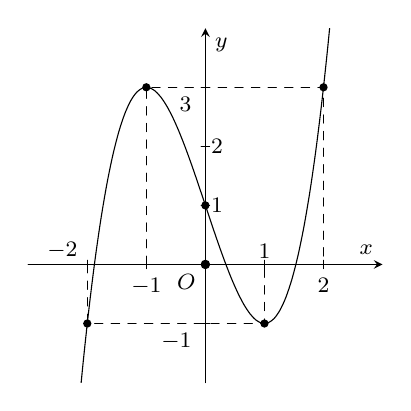
\begin{tikzpicture}[scale=0.75, font=\footnotesize, line join=round, line cap=round, >=stealth]
		\draw[->] (-3,0)--(3,0) node[above left]{\footnotesize $x$};
		\draw[->] (0,-2)--(0,4) node[below right] {\footnotesize $y$};
		\foreach \x in {1}	\draw[shift={(\x,0)},color=black] (0pt,2pt) -- (0pt,-2pt) node[above] {\footnotesize $\x$};
		\foreach \x in {-2}	\draw[shift={(\x,0)},color=black] (0pt,2pt) -- (0pt,-2pt) node[above left] {\footnotesize $\x$};
		\foreach \x in {-1,2}	\draw[shift={(\x,0)},color=black] (0pt,2pt) -- (0pt,-2pt) node[below] {\footnotesize $\x$};
		\foreach \y in {-1,3}		\draw[shift={(0,\y)},color=black] (2pt,0pt) -- (-2pt,0pt) node[below left] {\footnotesize $\y$};
		\foreach \y in {1,2}		\draw[shift={(0,\y)},color=black] (2pt,0pt) -- (-2pt,0pt) node[right] {\footnotesize $\y$};
		\filldraw (0,0) circle(2pt) node [below left] {\footnotesize $O$};
		\fill (-2,-1)circle(2pt) (-1,3)circle(2pt) (1,-1)circle(2pt) (2,3)circle(2pt) (0,1)circle(2pt);
		\begin{scope}
		\clip (-3,-2) rectangle (3,4);
		\draw[samples=100,smooth,variable=\x] plot (\x,{(\x)^3-3*(\x)+1});
		\end{scope}
		\draw[dashed] (-2,0)--(-2,-1)--(1,-1)--(1,0) (-1,0)--(-1,3)--(2,3)--(2,0) ;
		\end{tikzpicture}
	}
	\loigiai{
		Đặt $t=\pi^x$ $(t>0)$, phương trình đã cho trở thành $f(t)=\dfrac{m^2-1}{8}$. \hfill $(1)$\\
		Với mỗi $t>0$ cho ta duy nhất một nghiệm $x=\log_{\pi}t$.\\
		Vậy phương trình đã cho có hai nghiệm phân biệt khi và chỉ khi $(1)$ có đúng hai nghiệm $t>0$. Điều này xảy ra khi $-1<\dfrac{m^2-1}{8}<1\Leftrightarrow -3<m<3$.\\
		Vậy có $5$ số nguyên thỏa mãn.
	}%<MyLT1>
\end{ex}

% #3755 | Archive/SP_KhoLatex/ID6_old/2D2Y3-2.tex | mã gốc 2D2Y3-2
\begin{ex}%[Dự án VTED-2019]%[Thầy Hóa - Trần Nhân Kiệt]%[2D2Y3-2]
	Cho hai số thực với $b\neq 0$, $0<a\neq 1$. Khẳng định nào sau đây đúng?
	\haicot
	{$\log_ab^2=2\log_ab$}
	{$\log_ab^2=-2\log_ab$}
	{\True $\log_ab^2=2\log_a|b|$}
	{$\log_ab^2=-2\log_a|b|$}
	\loigiai{
		Do $b\neq 0$ nên $\log_ab^2=2\log_a|b|$.}
\end{ex}
